\PassOptionsToPackage{unicode=true}{hyperref} % options for packages loaded elsewhere
\PassOptionsToPackage{hyphens}{url}
%
\documentclass[11pt,ignorenonframetext,]{beamer}
\setbeamertemplate{caption}[numbered]
\setbeamertemplate{caption label separator}{: }
\setbeamercolor{caption name}{fg=normal text.fg}
\beamertemplatenavigationsymbolsempty
\usepackage{lmodern}
\usepackage{amssymb,amsmath}
\usepackage{ifxetex,ifluatex}
\usepackage{fixltx2e} % provides \textsubscript
\ifnum 0\ifxetex 1\fi\ifluatex 1\fi=0 % if pdftex
  \usepackage[T1]{fontenc}
  \usepackage[utf8]{inputenc}
  \usepackage{textcomp} % provides euro and other symbols
\else % if luatex or xelatex
  \usepackage{unicode-math}
  \defaultfontfeatures{Ligatures=TeX,Scale=MatchLowercase}
\fi
\usetheme[]{metropolis}
% use upquote if available, for straight quotes in verbatim environments
\IfFileExists{upquote.sty}{\usepackage{upquote}}{}
% use microtype if available
\IfFileExists{microtype.sty}{%
\usepackage[]{microtype}
\UseMicrotypeSet[protrusion]{basicmath} % disable protrusion for tt fonts
}{}
\IfFileExists{parskip.sty}{%
\usepackage{parskip}
}{% else
\setlength{\parindent}{0pt}
\setlength{\parskip}{6pt plus 2pt minus 1pt}
}
\usepackage{hyperref}
\hypersetup{
            pdftitle={Lecture 12},
            pdfborder={0 0 0},
            breaklinks=true}
\urlstyle{same}  % don't use monospace font for urls
\newif\ifbibliography
\usepackage{color}
\usepackage{fancyvrb}
\newcommand{\VerbBar}{|}
\newcommand{\VERB}{\Verb[commandchars=\\\{\}]}
\DefineVerbatimEnvironment{Highlighting}{Verbatim}{commandchars=\\\{\}}
% Add ',fontsize=\small' for more characters per line
\newenvironment{Shaded}{}{}
\newcommand{\AlertTok}[1]{\textcolor[rgb]{1.00,0.00,0.00}{\textbf{#1}}}
\newcommand{\AnnotationTok}[1]{\textcolor[rgb]{0.38,0.63,0.69}{\textbf{\textit{#1}}}}
\newcommand{\AttributeTok}[1]{\textcolor[rgb]{0.49,0.56,0.16}{#1}}
\newcommand{\BaseNTok}[1]{\textcolor[rgb]{0.25,0.63,0.44}{#1}}
\newcommand{\BuiltInTok}[1]{#1}
\newcommand{\CharTok}[1]{\textcolor[rgb]{0.25,0.44,0.63}{#1}}
\newcommand{\CommentTok}[1]{\textcolor[rgb]{0.38,0.63,0.69}{\textit{#1}}}
\newcommand{\CommentVarTok}[1]{\textcolor[rgb]{0.38,0.63,0.69}{\textbf{\textit{#1}}}}
\newcommand{\ConstantTok}[1]{\textcolor[rgb]{0.53,0.00,0.00}{#1}}
\newcommand{\ControlFlowTok}[1]{\textcolor[rgb]{0.00,0.44,0.13}{\textbf{#1}}}
\newcommand{\DataTypeTok}[1]{\textcolor[rgb]{0.56,0.13,0.00}{#1}}
\newcommand{\DecValTok}[1]{\textcolor[rgb]{0.25,0.63,0.44}{#1}}
\newcommand{\DocumentationTok}[1]{\textcolor[rgb]{0.73,0.13,0.13}{\textit{#1}}}
\newcommand{\ErrorTok}[1]{\textcolor[rgb]{1.00,0.00,0.00}{\textbf{#1}}}
\newcommand{\ExtensionTok}[1]{#1}
\newcommand{\FloatTok}[1]{\textcolor[rgb]{0.25,0.63,0.44}{#1}}
\newcommand{\FunctionTok}[1]{\textcolor[rgb]{0.02,0.16,0.49}{#1}}
\newcommand{\ImportTok}[1]{#1}
\newcommand{\InformationTok}[1]{\textcolor[rgb]{0.38,0.63,0.69}{\textbf{\textit{#1}}}}
\newcommand{\KeywordTok}[1]{\textcolor[rgb]{0.00,0.44,0.13}{\textbf{#1}}}
\newcommand{\NormalTok}[1]{#1}
\newcommand{\OperatorTok}[1]{\textcolor[rgb]{0.40,0.40,0.40}{#1}}
\newcommand{\OtherTok}[1]{\textcolor[rgb]{0.00,0.44,0.13}{#1}}
\newcommand{\PreprocessorTok}[1]{\textcolor[rgb]{0.74,0.48,0.00}{#1}}
\newcommand{\RegionMarkerTok}[1]{#1}
\newcommand{\SpecialCharTok}[1]{\textcolor[rgb]{0.25,0.44,0.63}{#1}}
\newcommand{\SpecialStringTok}[1]{\textcolor[rgb]{0.73,0.40,0.53}{#1}}
\newcommand{\StringTok}[1]{\textcolor[rgb]{0.25,0.44,0.63}{#1}}
\newcommand{\VariableTok}[1]{\textcolor[rgb]{0.10,0.09,0.49}{#1}}
\newcommand{\VerbatimStringTok}[1]{\textcolor[rgb]{0.25,0.44,0.63}{#1}}
\newcommand{\WarningTok}[1]{\textcolor[rgb]{0.38,0.63,0.69}{\textbf{\textit{#1}}}}
\usepackage{longtable,booktabs}
\usepackage{caption}
% These lines are needed to make table captions work with longtable:
\makeatletter
\def\fnum@table{\tablename~\thetable}
\makeatother
% Prevent slide breaks in the middle of a paragraph:
\widowpenalties 1 10000
\raggedbottom
\setbeamertemplate{part page}{
\centering
\begin{beamercolorbox}[sep=16pt,center]{part title}
  \usebeamerfont{part title}\insertpart\par
\end{beamercolorbox}
}
\setbeamertemplate{section page}{
\centering
\begin{beamercolorbox}[sep=12pt,center]{part title}
  \usebeamerfont{section title}\insertsection\par
\end{beamercolorbox}
}
\setbeamertemplate{subsection page}{
\centering
\begin{beamercolorbox}[sep=8pt,center]{part title}
  \usebeamerfont{subsection title}\insertsubsection\par
\end{beamercolorbox}
}
\AtBeginPart{
  \frame{\partpage}
}
\AtBeginSection{
  \ifbibliography
  \else
    \frame{\sectionpage}
  \fi
}
\AtBeginSubsection{
  \frame{\subsectionpage}
}
\setlength{\emergencystretch}{3em}  % prevent overfull lines
\providecommand{\tightlist}{%
  \setlength{\itemsep}{0pt}\setlength{\parskip}{0pt}}
\setcounter{secnumdepth}{0}

% set default figure placement to htbp
\makeatletter
\def\fps@figure{htbp}
\makeatother

\usepackage{geometry}
\usepackage{graphicx}

\usepackage{bbold}
\usepackage{lmodern}


\usepackage{url}		% produces hyperlinks

\usepackage{colortbl}	% allows for color usage in tables
\usepackage{multirow}	% allows for rows that span multiple rows in tables

\usepackage{color}          	% gives color options
\usepackage{xcolor}		% this package has a variety of color options

\usepackage{multicol}
\usepackage{textcomp}

\usepackage{setspace}
\usepackage{changepage}
\usepackage{isotope}

\singlespacing

%%%%%%%%%%%%%%%%
% Small code output
%%%%%%%%%%%%%%%%

%% change fontsize of R code

\makeatletter
\@ifundefined{Shaded}{\newenvironment{Shaded}{}{}}{}
\makeatother


\let\oldShaded\Shaded
\let\endoldShaded\endShaded
\renewenvironment{Shaded}{\footnotesize\begin{spacing}{0.9}\oldShaded}{\endoldShaded\end{spacing}}

%% change fontsize of output
\let\oldverbatim\verbatim
\let\endoldverbatim\endverbatim
\renewenvironment{verbatim}{\footnotesize\begin{spacing}{0.9}\oldverbatim}{\endoldverbatim\end{spacing}}


\newcommand{\tinyoutput}{
  \renewenvironment{Shaded}{\tiny\begin{spacing}{0.9}\oldShaded}{\endoldShaded\end{spacing}}
  \renewenvironment{verbatim}{\tiny\begin{spacing}{0.9}\oldverbatim}{\endoldverbatim\end{spacing}}
}

\newcommand{\scriptoutput}{
  \renewenvironment{Shaded}{\scriptsize\begin{spacing}{0.9}\oldShaded}{\endoldShaded\end{spacing}}
  \renewenvironment{verbatim}{\scriptsize\begin{spacing}{0.9}\oldverbatim}{\endoldverbatim\end{spacing}}
}

\newcommand{\footnoteoutput}{
  \renewenvironment{Shaded}{\footnotesize\begin{spacing}{0.9}\oldShaded}{\endoldShaded\end{spacing}}
  \renewenvironment{verbatim}{\footnotesize\begin{spacing}{0.9}\oldverbatim}{\endoldverbatim\end{spacing}}
}

%\newcommand{\verbatimfont}[1]{\renewcommand{\verbatim@font}{\ttfamily#1}}


%%%%%%%%%%%%%%%%
% Custom Colors
%%%%%%%%%%%%%%%%

\definecolor{redhl}{rgb}{0.98,0.29,0.28}
\definecolor{yellowhl}{rgb}{0.98,0.87,0.28}


\xdefinecolor{oiBlue}{rgb}{0.15, 0.35, 0.55}
\xdefinecolor{gray}{rgb}{0.5, 0.5, 0.5}
\xdefinecolor{darkGray}{rgb}{0.3, 0.3, 0.3}
\xdefinecolor{darkerGray}{rgb}{0.2, 0.2, 0.2}
\xdefinecolor{rubineRed}{rgb}{0.89,0,0.30}
\xdefinecolor{linkCol}{rgb}{0.11,0.49,0.95}	
\xdefinecolor{irishGreen}{rgb}{0,0.60,0}	
\xdefinecolor{darkturquoise}{rgb}{0.44, 0.58, 0.86}
\definecolor{lightGreen}{rgb}{0.533,0.765,0.42}
%\xdefinecolor{hlblue}{rgb}{0.051,0.65,1}
\xdefinecolor{hlblue}{rgb}{ 0.055, 0.639, 0.831}
\definecolor{light}{rgb}{.337,.608,.741}
\definecolor{dark}{rgb}{.337,.608,.741}

\definecolor{cpink}{rgb}{0.93, 0.23, 0.51}

%%%%%%%%%%%%%%%%
% Custom Commands
%%%%%%%%%%%%%%%%

% text colors
\newcommand{\red}[1]{\textit{\textcolor{rubineRed}{#1}}}
\newcommand{\orange}[1]{\textit{\textcolor{orange}{#1}}}
\newcommand{\pink}[1]{\textit{\textcolor{rubineRed!90!white!50}{#1}}}
\newcommand{\green}[1]{\textit{\textcolor{irishGreen}{#1}}}
\newcommand{\blue}[1]{\textit{\textcolor{darkturquoise}{#1}}}
\newcommand{\light}[1]{\textcolor{light}{\textbf{#1}}}
\newcommand{\dark}[1]{\textcolor{dark}{#1}}
\newcommand{\gray}[1]{\textcolor{gray}{#1}}


% mail
\newcommand{\mail}[1]{\href{mailto:#1}{\textit{\textcolor{linkCol}{#1}}}}

% highlighting: hl, hlGr, mathhl
\newcommand{\hl}[1]{\textit{\textcolor{hlblue}{#1}}}
\newcommand{\hlGr}[1]{\textit{\textcolor{lightGreen}{#1}}}
\newcommand{\hlRd}[1]{\textit{\textcolor{rubineRed}{#1}}}
\newcommand{\mathhl}[1]{\textcolor{hlblue}{\ensuremath{#1}}}
\newcommand{\hlr}[1]{\fcolorbox{redhl}{white}{$\displaystyle #1$}}
\newcommand{\hly}[1]{\fcolorbox{yellowhl}{white}{$\displaystyle #1$}}


\newcommand{\vvfill}{\vskip0pt plus 1filll}

\DeclareMathOperator*{\argmin}{arg\,min}
\DeclareMathOperator*{\argmax}{arg\,max}

\title{Lecture 12}
\providecommand{\subtitle}[1]{}
\subtitle{Gaussian Process Models}
\date{3/01/2018}

\begin{document}
\frame{\titlepage}

\hypertarget{multivariate-normal}{%
\section{Multivariate Normal}\label{multivariate-normal}}

\begin{frame}[t]{%
\protect\hypertarget{multivariate-normal-distribution}{%
Multivariate Normal Distribution}}

For an \(n\)-dimension multivate normal distribution with covariance
\(\symbf{\Sigma}\) (positive semidefinite) can be written as

\[
\underset{n \times 1}{\symbf{Y}} \sim N(\underset{n \times 1}{\symbf{\mu}}, \; \underset{n \times n}{\symbf{\Sigma}}) \text{   where   } \{\symbf{\Sigma}\}_{ij} = \sigma^2_{ij} = \rho_{ij} \, \sigma_{i} \, \sigma_{j}
\]

\vspace{2mm}

\[
\begin{pmatrix}
Y_1\\ \vdots\\ Y_n
\end{pmatrix}
\sim N\left(
\begin{pmatrix}
\mu_1\\ \vdots\\ \mu_n
\end{pmatrix}, \,
\begin{pmatrix}
\rho_{11}\sigma_1\sigma_1 & \cdots & \rho_{1n}\sigma_1\sigma_n \\
\vdots & \ddots & \vdots \\
\rho_{n1}\sigma_n\sigma_1 & \cdots & \rho_{nn}\sigma_n\sigma_n \\
\end{pmatrix}
\right)
\]

\end{frame}

\begin{frame}[t]{%
\protect\hypertarget{density}{%
Density}}

For the \(n\) dimensional multivate normal given on the last slide, its
density is given by

\[
(2\pi)^{-n/2} \; \det(\symbf{\Sigma})^{-1/2} \; \exp{\left(-\frac{1}{2} \underset{1 \times n}{(\symbf{Y}-\symbf{\mu})'} \underset{n \times n}{\symbf{\Sigma}^{-1}} \underset{n \times 1}{(\symbf{Y}-\symbf{\mu})}\right)} 
\]

and its log density is given by

\[
-\frac{n}{2} \log 2\pi - \frac{1}{2} \log \det(\symbf{\Sigma}) - -\frac{1}{2} \underset{1 \times n}{(\symbf{Y}-\symbf{\mu})'} \underset{n \times n}{\symbf{\Sigma}^{-1}} \underset{n \times 1}{(\symbf{Y}-\symbf{\mu})}
\]

\end{frame}

\begin{frame}[t]{%
\protect\hypertarget{sampling}{%
Sampling}}

To generate draws from an \(n\)-dimensional multivate normal with mean
\(\symbf{\mu}\) and covariance matrix \(\symbf{\Sigma}\),

\vspace{4mm}

\pause

\begin{itemize}
\tightlist
\item
  Find a matrix \(\symbf{A}\) such that
  \(\symbf{\Sigma} = \symbf{A}\,\symbf{A}^t\), most often we use
  \(\symbf{A} = \text{Chol}(\symbf{\Sigma})\)
\end{itemize}

\pause

\vspace{2mm}

\begin{itemize}
\tightlist
\item
  Draw \(n\) iid unit normals (\(\mathcal{N}(0,1)\)) as \(\symbf{z}\)
\end{itemize}

\pause

\vspace{2mm}

\begin{itemize}
\tightlist
\item
  Construct multivariate normal draws using
  \[ \symbf{Y} = \symbf{\mu} + \symbf{A} \, \symbf{z} \]
\end{itemize}

\end{frame}

\begin{frame}{%
\protect\hypertarget{bivariate-example}{%
Bivariate Example}}

\scriptsize

\[ \symbf{\mu} = \begin{pmatrix}0 \\ 0\end{pmatrix} \qquad \symbf{\Sigma} = \begin{pmatrix}1 & \rho \\ \rho & 1 \end{pmatrix}\]

\begin{center}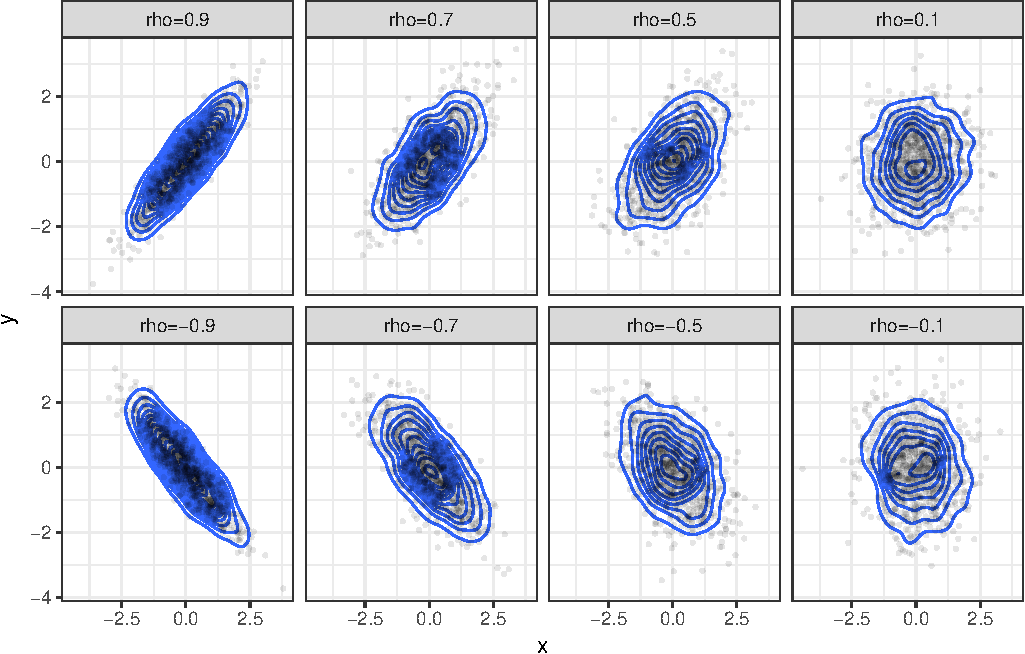
\includegraphics[width=\textwidth]{Lec12_files/figure-beamer/unnamed-chunk-1-1} \end{center}

\end{frame}

\begin{frame}{%
\protect\hypertarget{marginal-distributions}{%
Marginal distributions}}

\small

\textbf{Proposition} - For an \(n\)-dimensional multivate normal with
mean \(\symbf{\mu}\) and covariance matrix \(\symbf{\Sigma}\), any
marginal or conditional distribution of the \(y\)’s will also
(multivariate) normal.

\pause

\vspace{2mm}

For a univariate marginal distribution,
\[ y_i = \mathcal{N}(\mu_i,\,\gamma_{ii}) \]

\pause

For a bivariate marginal distribution,
\[ \symbf{y}_{ij} = \mathcal{N}\left( \begin{pmatrix}\mu_i \\ \mu_j \end{pmatrix},\; \begin{pmatrix} \gamma_{ii} & \gamma_{ij} \\ \gamma_{ji} & \gamma_{jj} \end{pmatrix} \right) \]

\pause

For a \(k\)-dimensional marginal distribution,

\[ 
\symbf{y}_{i_1,\cdots,i_k} = 
  \mathcal{N}\left( 
    \begin{pmatrix}\mu_{i_1} \\ \vdots \\ \mu_j \end{pmatrix},\; 
    \begin{pmatrix} 
      \gamma_{i_1i_1}  & \cdots & \gamma_{i_1 i_k} \\ 
      \vdots           & \ddots & \vdots \\
      \gamma_{i_k i_1} & \cdots & \gamma_{i_k i_k} \end{pmatrix} 
  \right) 
\]

\end{frame}

\begin{frame}[t]{%
\protect\hypertarget{conditional-distributions}{%
Conditional Distributions}}

If we partition the \(n\)-dimensions into two pieces such that
\(\symbf{Y} = (\symbf{Y}_1,\, \symbf{Y}_2)^t\) then \footnotesize \[
\underset{n \times 1}{\symbf{Y}} \sim \mathcal{N}\left(
  \underset{n \times 1}{\begin{pmatrix}\symbf{\mu}_1 \\ \symbf{\mu}_2\end{pmatrix}},\, 
  \underset{n \times n}{\begin{pmatrix} 
    \symbf{\Sigma}_{11} & \symbf{\Sigma}_{12} \\ 
    \symbf{\Sigma}_{21} & \symbf{\Sigma}_{22} 
  \end{pmatrix}}
\right)
\] \[ \begin{aligned}
\underset{k \times 1}{\symbf{Y}_1} &\sim \mathcal{N}(\underset{k \times 1}{\symbf{\mu}_1},\, \underset{k \times k}{\symbf{\Sigma}_{11}}) \\ 
\underset{n-k \times 1}{\symbf{Y}_2} &\sim \mathcal{N}(\underset{n-k \times 1}{\symbf{\mu}_2},\, \underset{n-k \times n-k}{\symbf{\Sigma}_{22}})
\end{aligned} \]

\pause

\normalsize \vspace{2mm}

then the conditional distributions are given by

\footnotesize

\[\begin{aligned}
\symbf{Y_1} ~|~ \symbf{Y}_2 = \symbf{a} ~&\sim \mathcal{N}(\symbf{\mu_1} + \symbf{\Sigma_{12}} \, \symbf{\Sigma_{22}}^{-1} \, (\symbf{a} - \symbf{\mu_2}),~ \symbf{\Sigma_{11}}-\symbf{\Sigma_{12}}\,\symbf{\Sigma_{22}}^{-1} \, \symbf{\Sigma_{21}}) \\
\\
\symbf{Y_2} ~|~ \symbf{Y}_1 = \symbf{b} ~&\sim \mathcal{N}(\symbf{\mu_2} + \symbf{\Sigma_{21}} \, \symbf{\Sigma_{11}}^{-1} \, (\symbf{b} - \symbf{\mu_1}),~ \symbf{\Sigma_{22}}-\symbf{\Sigma_{21}}\,\symbf{\Sigma_{11}}^{-1} \, \symbf{\Sigma_{21}})
\end{aligned}\]

\end{frame}

\begin{frame}[t]{%
\protect\hypertarget{gaussian-processes}{%
Gaussian Processes}}

From Shumway,

\vspace{5mm}

\begin{quote}
A process, \(\symbf{Y} = \{Y(t) ~:~ t \in T\}\), is said to be a
Gaussian process if all possible finite dimensional vectors
\(\symbf{y} = (y_{t_1},y_{t_2},...,y_{t_n})^t\), for every collection of
time points \(t_1, t_2, \ldots , t_n\), and every positive integer
\(n\), have a multivariate normal distribution.
\end{quote}

\pause

So far we have only looked at examples of time series where \(T\) is
discete (and evenly spaces \& contiguous), it turns out things get a lot
more interesting when we explore the case where \(T\) is defined on a
\emph{continuous} space (e.g. \(\mathbb{R}\) or some subset of
\(\mathbb{R}\)).

\end{frame}

\hypertarget{gaussian-process-regression}{%
\section{Gaussian Process
Regression}\label{gaussian-process-regression}}

\begin{frame}[t]{%
\protect\hypertarget{parameterizing-a-gaussian-process}{%
Parameterizing a Gaussian Process}}

Imagine we have a Gaussian process defined such that
\(\symbf{Y} = \{Y(t) ~:~ t \in [0,1]\}\),

\pause

\begin{itemize}
\tightlist
\item
  We now have an uncountably infinite set of possible \(Y(t)\)s.
\end{itemize}

\pause

\begin{itemize}
\tightlist
\item
  We will only have a (small) finite number of observations
  \(Y(t_1), \ldots, Y(t_n)\) with which to say something useful about
  this infinite dimension process.
\end{itemize}

\pause

\begin{itemize}
\tightlist
\item
  The unconstrained covariance matrix for the observed data can have up
  to \(n(n+1)/2\) unique values\(^*\)
\end{itemize}

\pause

\begin{itemize}
\item
  Necessary to make some simplifying assumptions:

  \begin{itemize}
  \item
    Stationarity
  \item
    Simple parameterization of \(\Sigma\)
  \end{itemize}
\end{itemize}

\end{frame}

\begin{frame}{%
\protect\hypertarget{covariance-functions}{%
Covariance Functions}}

More on these next week, but for now some simple / common examples

\pause

Exponential Covariance:
\[ \Sigma(y_{t},y_{t'}) = \sigma^2 \exp\big(-|t-t'| \; l\,\big) \]

\pause

Squared Exponential Covariance:
\[ \Sigma(y_{t},y_{t'}) = \sigma^2 \exp\big(-(|t-t'| \; l\,)^2\big) \]

\pause

Powered Exponential Covariance (\(p \in (0,2]\)):
\[ \Sigma(y_{t},y_{t'}) = \sigma^2 \exp\big(-(|t-t'| \; l\,)^p\big) \]

\end{frame}

\begin{frame}{%
\protect\hypertarget{covariance-function---correlation-decay}{%
Covariance Function - Correlation Decay}}

\begin{center}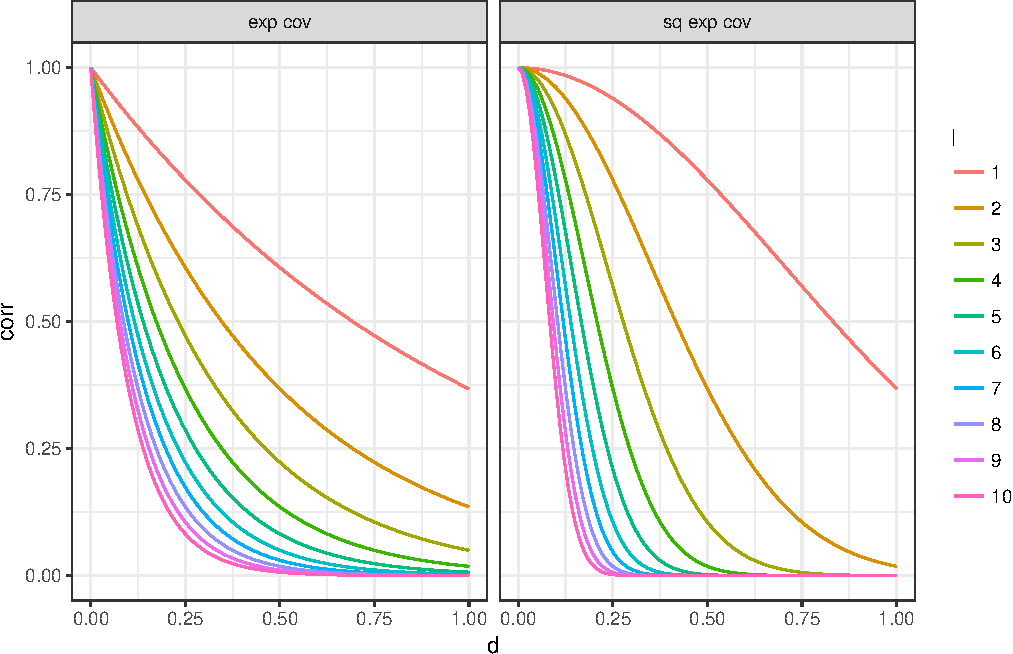
\includegraphics[width=\textwidth]{Lec12_files/figure-beamer/unnamed-chunk-2-1} \end{center}

\end{frame}

\begin{frame}{%
\protect\hypertarget{example}{%
Example}}

\begin{center}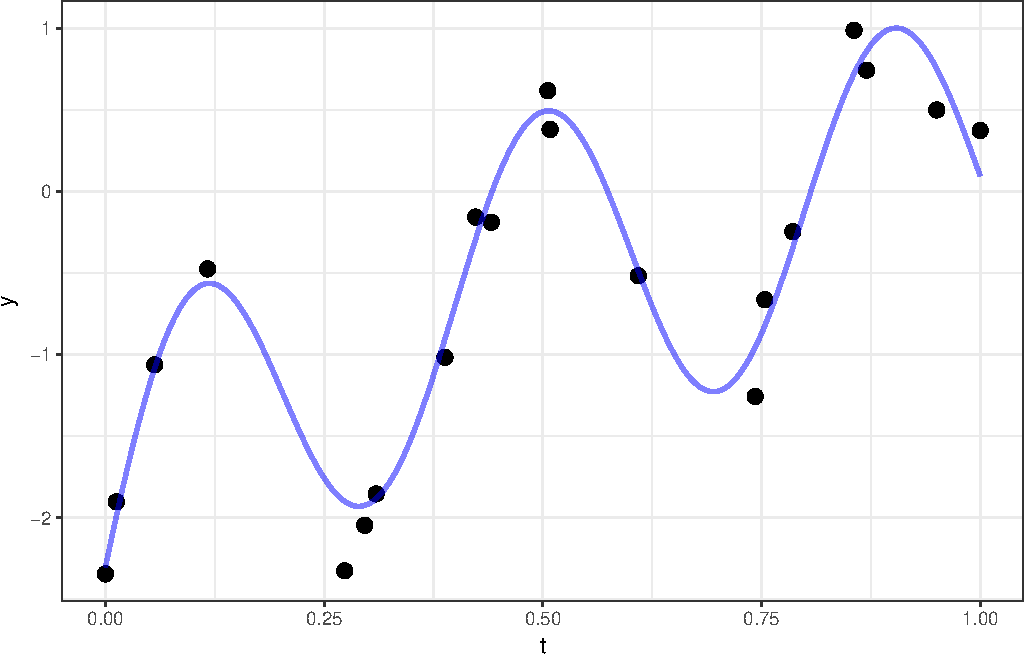
\includegraphics[width=\textwidth]{Lec12_files/figure-beamer/unnamed-chunk-3-1} \end{center}

\end{frame}

\begin{frame}[t]{%
\protect\hypertarget{prediction}{%
Prediction}}

Our example has 15 observations which we would like to use as the basis
for predicting \(Y_t\) at other values of \(t\) (say a grid of values
from 0 to 1).

\vspace{3mm}

\pause

For now lets use a square exponential covariance with \(\sigma^2 = 10\)
and \(l=10\)

\vspace{3mm}

\pause

We therefore want to sample from \(\symbf{Y}_{pred} | \symbf{Y}_{obs}\).

\[\symbf{Y}_{pred} ~|~ \symbf{Y}_{obs} = \symbf{y} ~\sim \mathcal{N}(\symbf{\Sigma}_{po} \, \symbf{\Sigma}_{obs}^{-1} \, \symbf{y},~ \symbf{\Sigma_{pred}}-\symbf{\Sigma}_{po}\,\symbf{\Sigma}_{pred}^{-1} \, \symbf{\Sigma}_{op})\]

\end{frame}

\begin{frame}{%
\protect\hypertarget{draw-1}{%
Draw 1}}

\begin{center}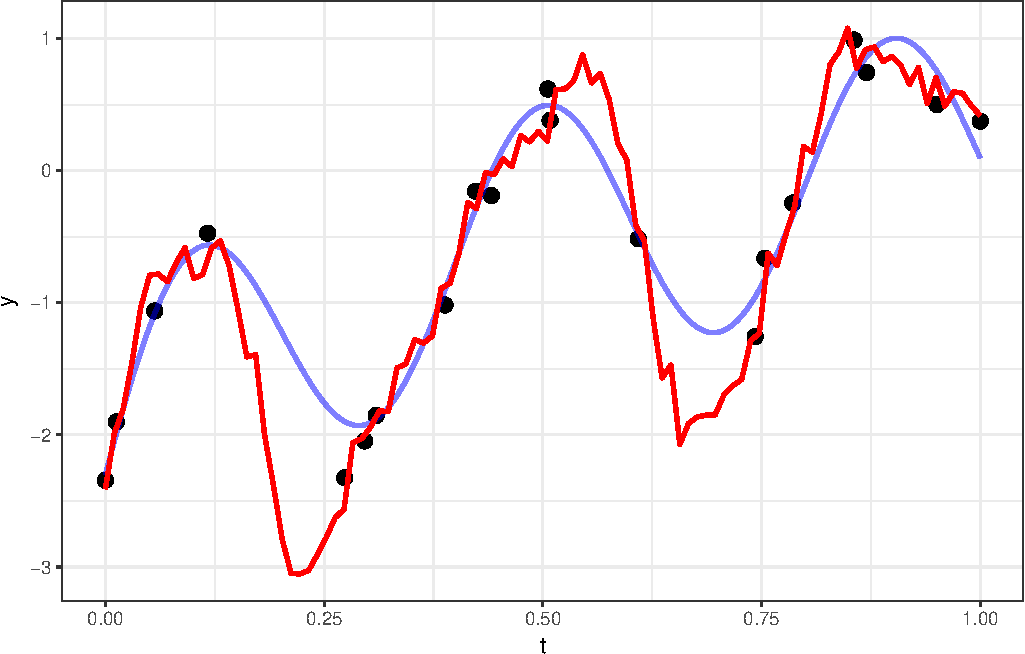
\includegraphics[width=\textwidth]{Lec12_files/figure-beamer/unnamed-chunk-5-1} \end{center}

\end{frame}

\begin{frame}{%
\protect\hypertarget{draw-2}{%
Draw 2}}

\begin{center}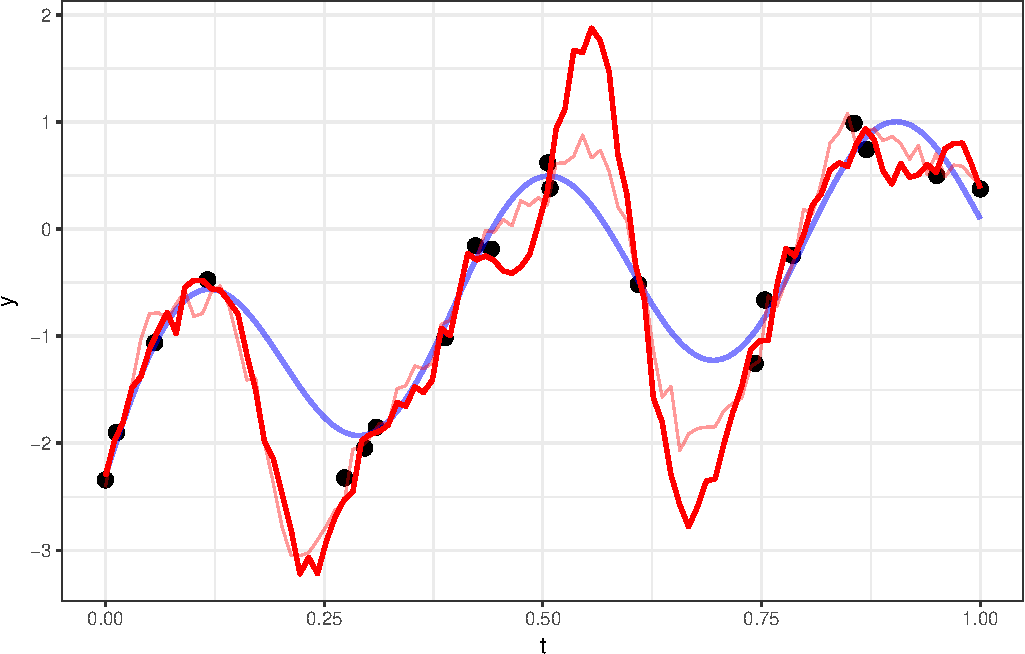
\includegraphics[width=\textwidth]{Lec12_files/figure-beamer/unnamed-chunk-6-1} \end{center}

\end{frame}

\begin{frame}{%
\protect\hypertarget{draw-3}{%
Draw 3}}

\begin{center}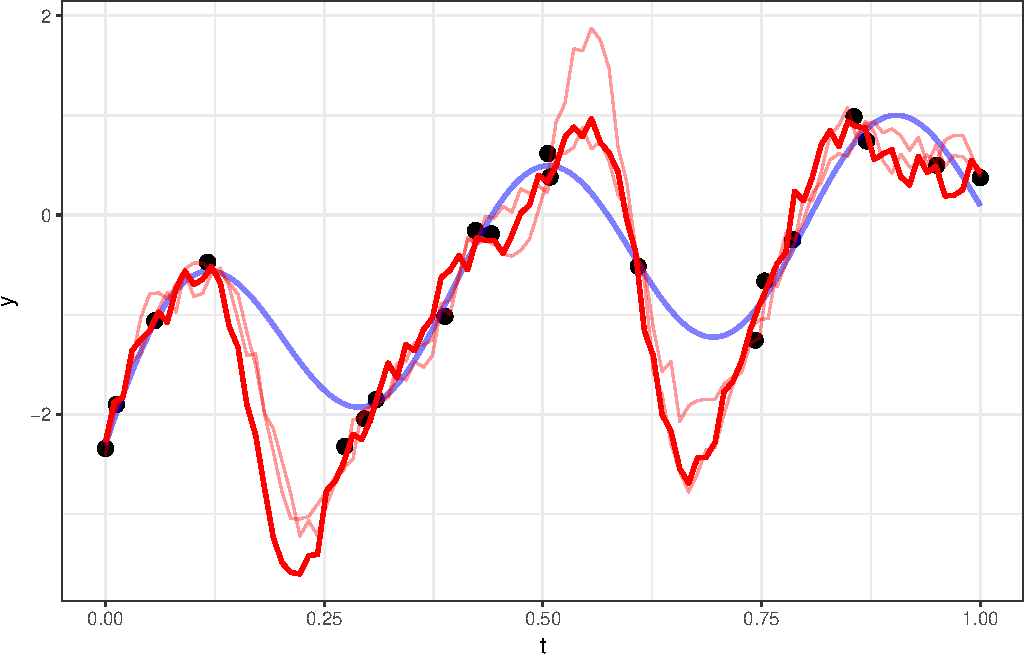
\includegraphics[width=\textwidth]{Lec12_files/figure-beamer/unnamed-chunk-7-1} \end{center}

\end{frame}

\begin{frame}{%
\protect\hypertarget{draw-4}{%
Draw 4}}

\begin{center}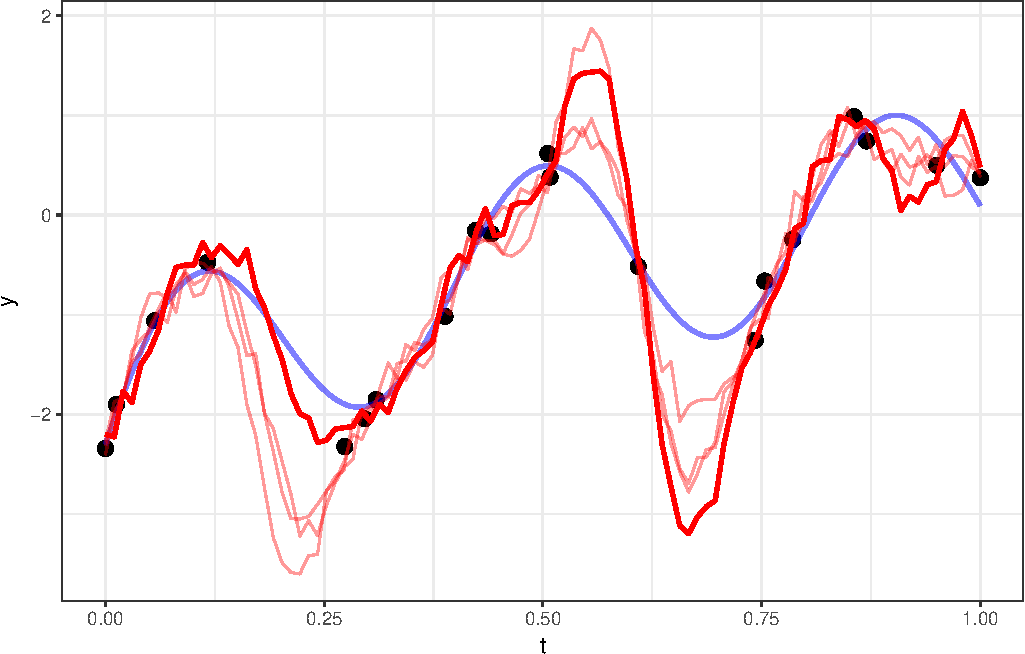
\includegraphics[width=\textwidth]{Lec12_files/figure-beamer/unnamed-chunk-8-1} \end{center}

\end{frame}

\begin{frame}{%
\protect\hypertarget{draw-5}{%
Draw 5}}

\begin{center}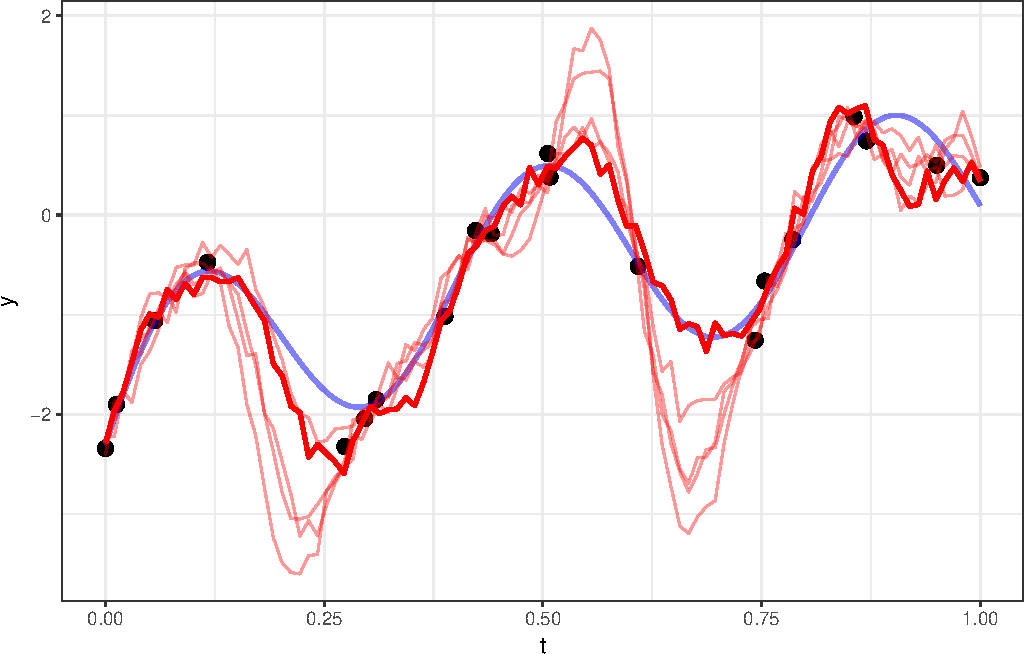
\includegraphics[width=\textwidth]{Lec12_files/figure-beamer/unnamed-chunk-9-1} \end{center}

\end{frame}

\begin{frame}{%
\protect\hypertarget{many-draws-later}{%
Many draws later}}

\begin{center}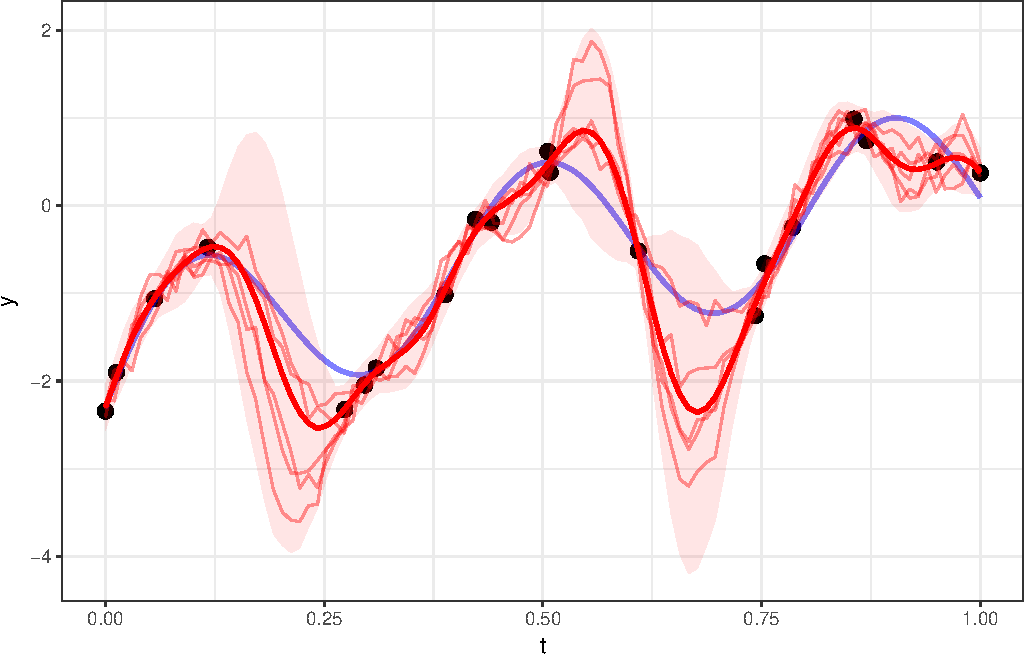
\includegraphics[width=\textwidth]{Lec12_files/figure-beamer/unnamed-chunk-10-1} \end{center}

\end{frame}

\begin{frame}{%
\protect\hypertarget{exponential-covariance}{%
Exponential Covariance}}

\begin{center}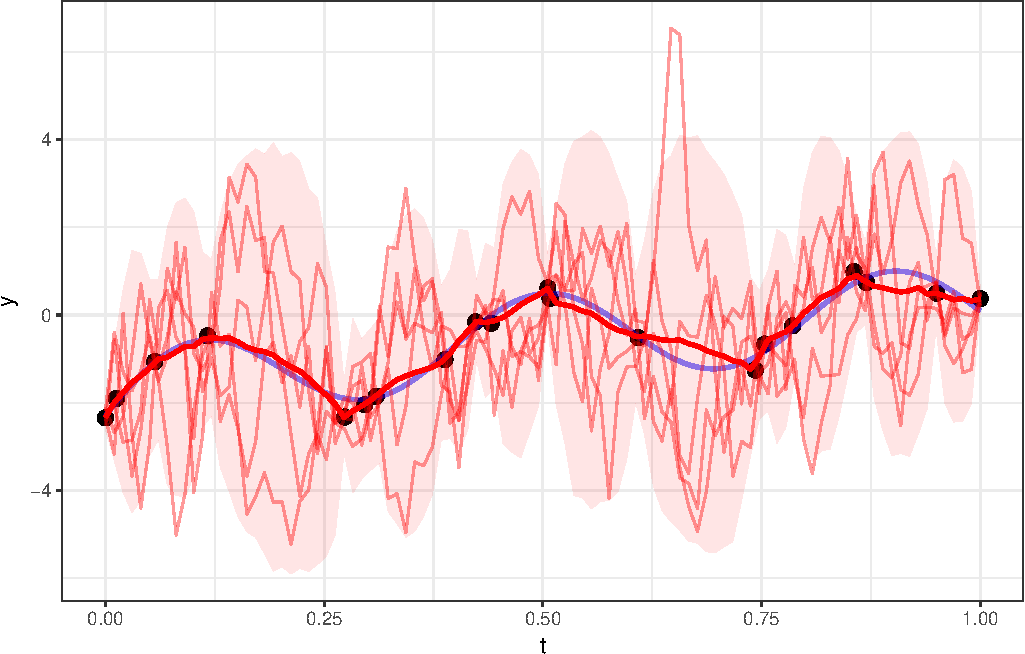
\includegraphics[width=\textwidth]{Lec12_files/figure-beamer/unnamed-chunk-11-1} \end{center}

\end{frame}

\begin{frame}{%
\protect\hypertarget{powered-exponential-covariance-p1.5}{%
Powered Exponential Covariance (\(p=1.5\))}}

\begin{center}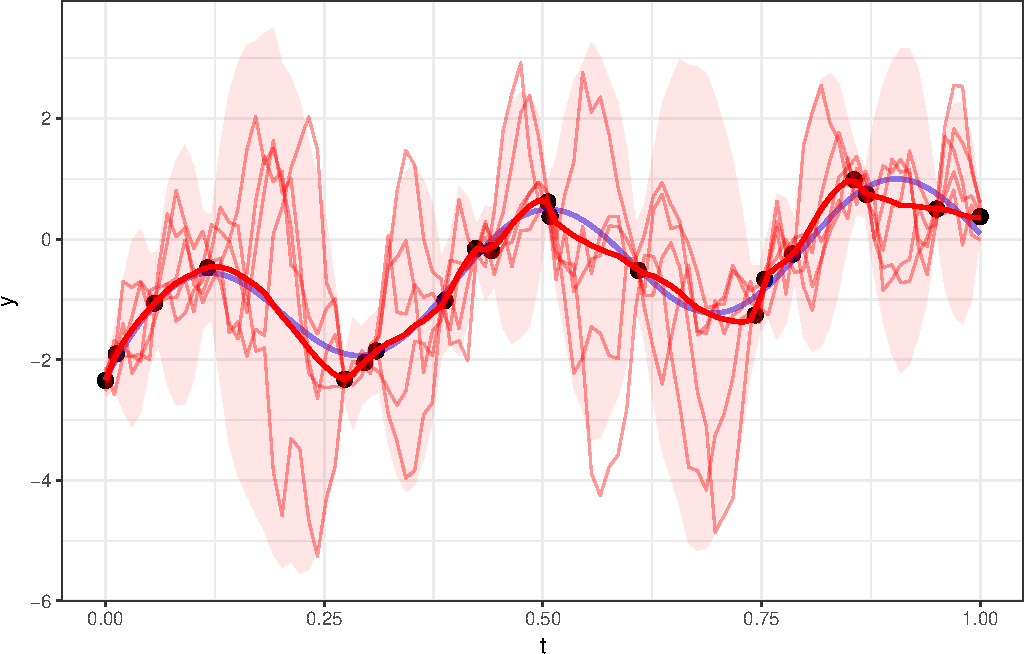
\includegraphics[width=\textwidth]{Lec12_files/figure-beamer/unnamed-chunk-12-1} \end{center}

\end{frame}

\begin{frame}{%
\protect\hypertarget{back-to-the-square-exponential}{%
Back to the square exponential}}

\begin{center}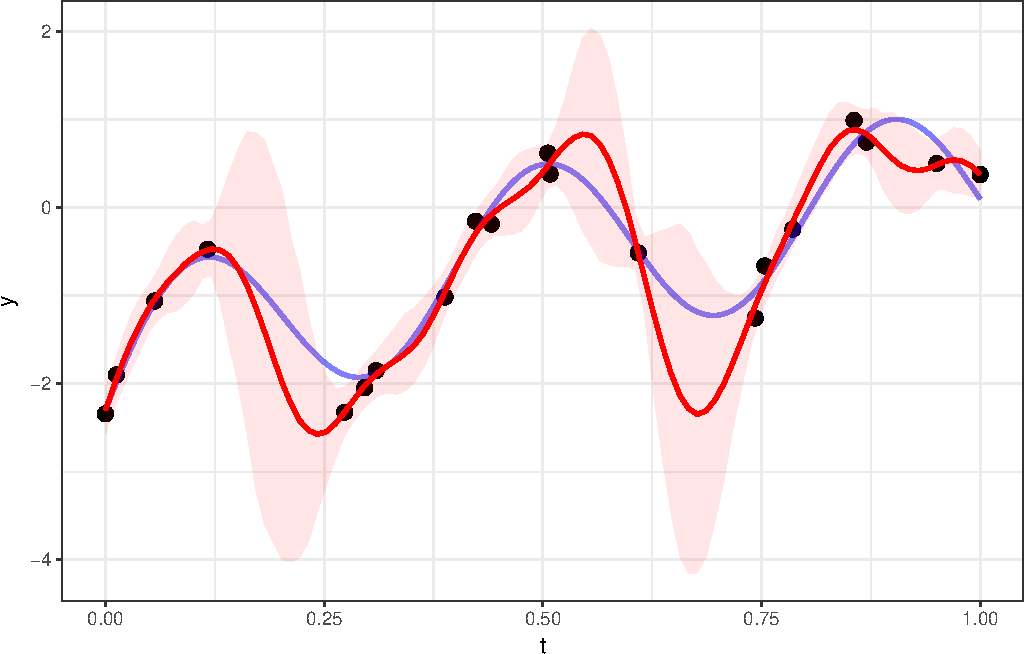
\includegraphics[width=\textwidth]{Lec12_files/figure-beamer/unnamed-chunk-13-1} \end{center}

\end{frame}

\begin{frame}{%
\protect\hypertarget{changing-the-range-l}{%
Changing the range (\(l\))}}

\begin{center}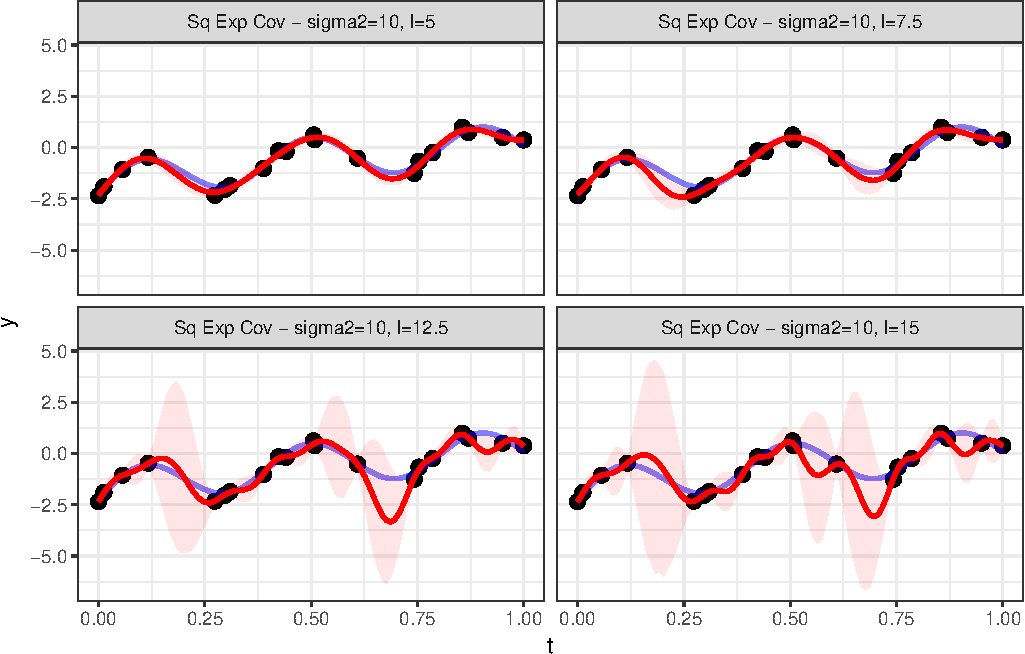
\includegraphics[width=\textwidth]{Lec12_files/figure-beamer/unnamed-chunk-14-1} \end{center}

\end{frame}

\begin{frame}[t]{%
\protect\hypertarget{effective-range}{%
Effective Range}}

For the square exponential covariance \[ \begin{aligned} 
Cov(d) &= \sigma^2 \exp\left(-(l \cdot d)^2\right) \\
Corr(d) &= \exp\left(-(l \cdot d)^2\right)
\end{aligned} \]

we would like to know, for a given value of \(l\), beyond what distance
apart must observations be to have a correlation less than \(0.05\)?

\end{frame}

\begin{frame}{%
\protect\hypertarget{changing-the-scale-sigma2}{%
Changing the scale (\(\sigma^2\))}}

\begin{center}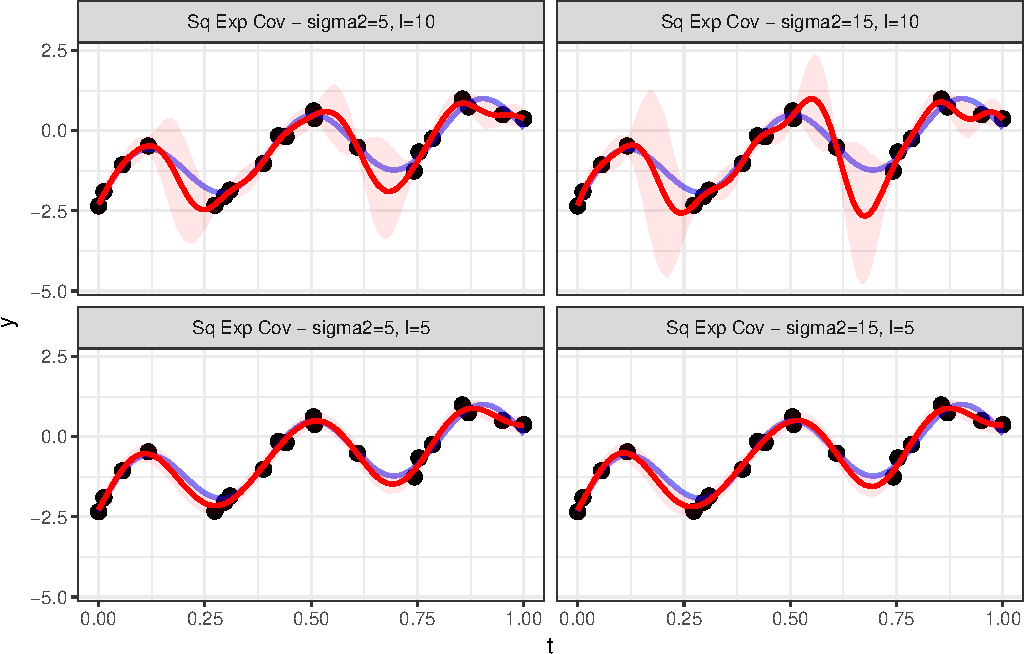
\includegraphics[width=\textwidth]{Lec12_files/figure-beamer/unnamed-chunk-15-1} \end{center}

\end{frame}

\begin{frame}[fragile]{%
\protect\hypertarget{fitting}{%
Fitting}}

\begin{Shaded}
\begin{Highlighting}[]
\NormalTok{gp_sq_exp_model =}\StringTok{ "model\{}
\StringTok{  y ~ dmnorm(mu, inverse(Sigma))}

\StringTok{  for (i in 1:N) \{}
\StringTok{    mu[i] <- 0}
\StringTok{  \}}

\StringTok{  for (i in 1:(N-1)) \{}
\StringTok{    for (j in (i+1):N) \{}
\StringTok{      Sigma[i,j] <- sigma2 * exp(- pow(l*d[i,j],2))}
\StringTok{      Sigma[j,i] <- Sigma[i,j]}
\StringTok{    \}}
\StringTok{  \}}

\StringTok{  for (k in 1:N) \{}
\StringTok{    Sigma[k,k] <- sigma2 + 0.01}
\StringTok{  \}}

\StringTok{  sigma2   ~ dlnorm(0, 1)}
\StringTok{  l        ~ dt(0, 2.5, 1) T(0,) # Half-cauchy(0,2.5)}
\StringTok{\}"}
\end{Highlighting}
\end{Shaded}

\end{frame}

\begin{frame}{%
\protect\hypertarget{trace-plots}{%
Trace plots}}

\begin{center}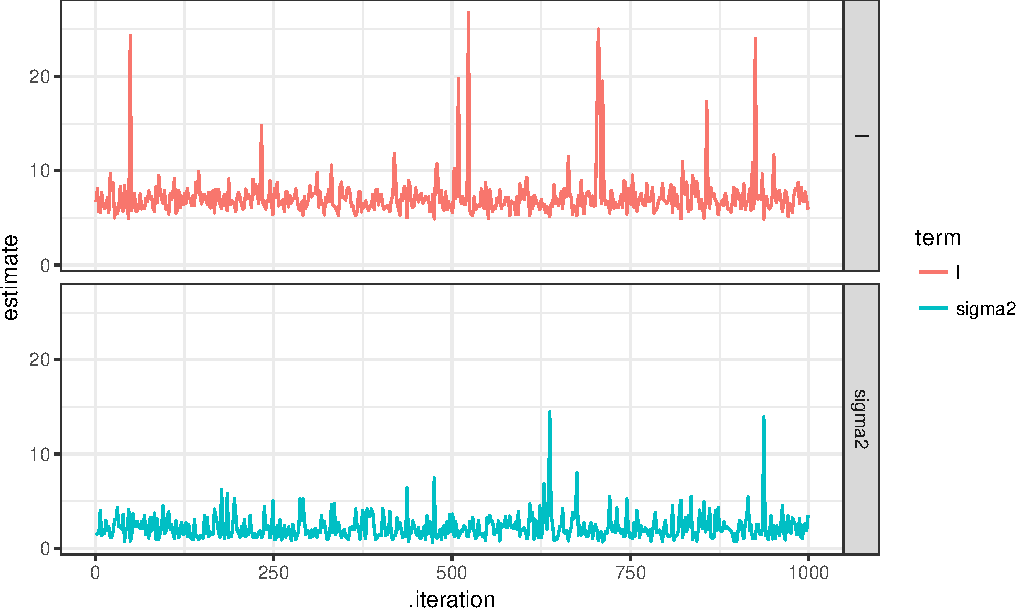
\includegraphics[width=\textwidth]{Lec12_files/figure-beamer/unnamed-chunk-18-1} \end{center}

\footnotesize

\begin{longtable}[]{@{}lrrrr@{}}
\toprule
param & post\_mean & post\_med & post\_lower &
post\_upper\tabularnewline
\midrule
\endhead
l & 7.21 & 6.79 & 5.23 & 10.95\tabularnewline
sigma2 & 2.18 & 1.86 & 0.84 & 5.24\tabularnewline
\bottomrule
\end{longtable}

\end{frame}

\begin{frame}{%
\protect\hypertarget{fitted-models}{%
Fitted models}}

\begin{center}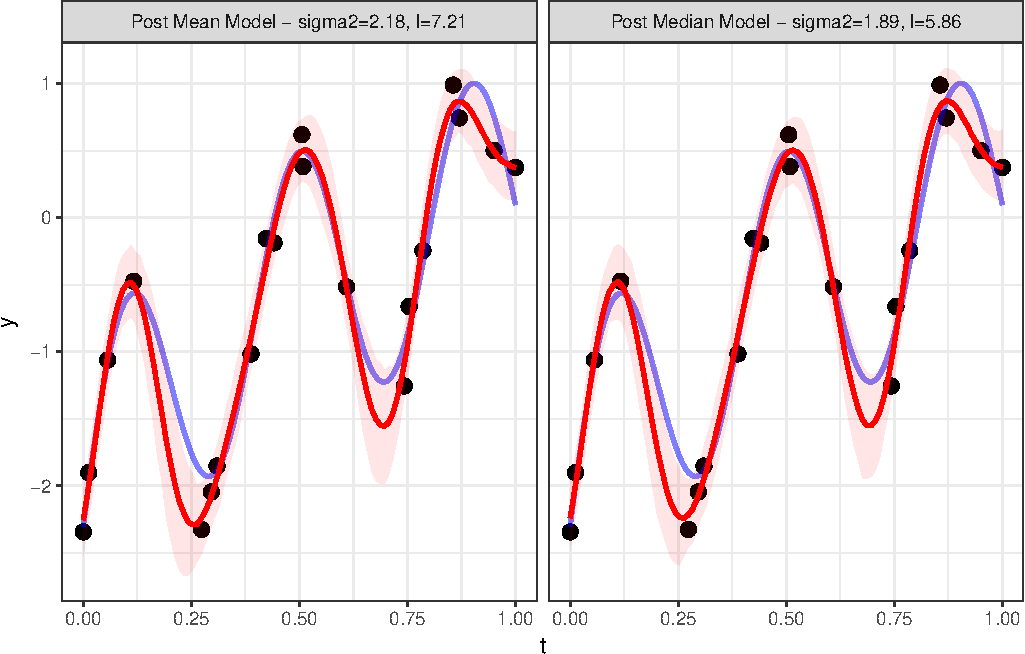
\includegraphics[width=\textwidth]{Lec12_files/figure-beamer/unnamed-chunk-20-1} \end{center}

\end{frame}

\begin{frame}{%
\protect\hypertarget{forcasting}{%
Forcasting}}

\begin{center}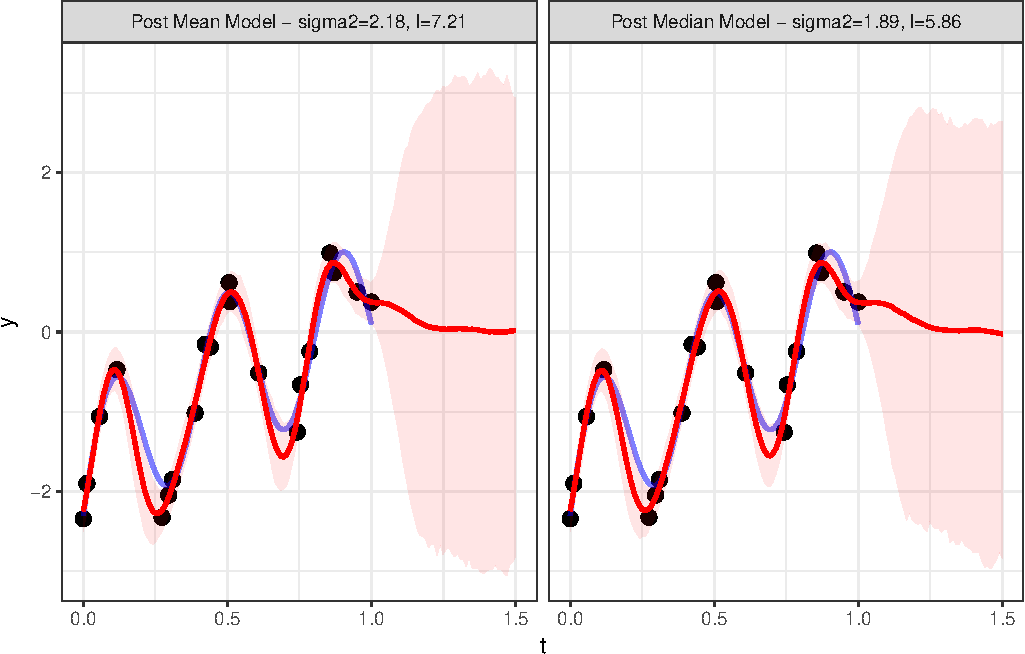
\includegraphics[width=\textwidth]{Lec12_files/figure-beamer/unnamed-chunk-21-1} \end{center}

\end{frame}

\end{document}
